% !TeX root = ../main.tex
% Add the above to each chapter to make compiling the PDF easier in some editors.

\chapter{Software Application}\label{Software Application}

\section{Methodology}
The main focus is to develop a low-cost mobile system to locate and examine veins. As one can infer from the design of the hardware extension from the previous chapter, the cost of the hardware components is mainly the cost of a normal webcam, NIR-pass filter, a PCB breadboard and a set of NIR LEDs. Obviously, the cost of these elements is very low (under 30 Euros). The second component is the software application. In order to maintain the low-cost constraint, the software application must be run on normal android mobiles or tablets. Not on special hardware or expensive embedded systems.

\subsection{Control of Hardware Extension}

The hardware extension is connected as a peripheral to an android device. In that sense, the android device takes over control of the hardware peripheral in somehow. This control can be described as power control and camera control.

\subsubsection{Power Control}
Only a single connection via OTG cable is needed. Data and power are then transferred using the data and power pins of the OTG connection respectively. Power is supplied whenever the OTG cable is plugged in. No programmable way for cutting off power was implemented. Because turning off the host port’s power needs write permission on the \texttt{/sys} directory and this cannot be acquired without root. The application is developed to be fully runnable on not rooted devices, so it requires no root access. For these reasons, controlling the OTG connection programmatically was out of the scope of this project. Of course, a physical switch can be also added on the whole circuit to turn the system on or off. 

\subsubsection{Camera Control}

A third-party library, UVC Camera library, was used in this project to enable the android device to communicate with the webcam. UVC Camera supports variety of camera properties control like brightness, contrast, focus control and more, given that the camera itself supports those. Support is indicated by flags that the camera provides. Control of such properties can be done in the C++ side. Signals are sent from the module to the camera to change sensor values. For example, brightness and contrast control were added in the project. In this case, brightness and contrast are controlled by changing some sensor values, without the need of using image processing at all.


As per the UVC specification, if the auto setting is supported and set to the on state, the device will provide automatic focus adjustment, and read requests will reflect the automatically set value \parencite{uvcCamera}. Attempts to programmatically set the Focus control are ignored when auto mode is set. When the UVC Camera library detects an autofocus support in a connected webcam, it uses it and sets the autofocus mode.



\subsection{Vein Visualization Enhancement}

In our setting, raw videos that come directly from the NIR camera provide good visualization of the vein’s structure and their pattern. However, they contain some fuzzy and noisy areas caused by shades or hairs.

Veins visualization can be enhanced more using image processing or machine learning.
Videos received by a camera are made up from a succession of still frames and are then played one after the other several times a second. Image enhancement algorithms can be applied on each frame separately each time a new frame arrives from the camera. The result is then displayed in the real time on the screen.

\subsubsection{Machine Learning}

The term machine learning refers to the automated detection of meaningful patterns in data \parencite{machineLearning}.
Using machine learning algorithms can be beneficial in automatically recognizing veins and highlighting or colouring them, and thus, making the task even easier for the operator. An algorithm is trained on a dataset of different images in a similar or same setting as in the practical case. It “learns” then how a vein could look like and can extract it from a new given image. The task of finding a vein in an image using machine learning is not hard and totally feasible as much more complex tasks are accomplished in this field like face localization \parencite{faceLocal} and active object localization \parencite{objectLocal} and they give great results and performance. However, using machine learning requires access to a reasonably big dataset to train the algorithm, which means an images dataset, where each image is taken in the same or similar setting as our setting. Such dataset is unfortunately unavailable.
Moreover, if the image provides good contrast of the veins pattern, there is no need for such automatic recognition because it will be then an easy task for the operator to visually recognize it. For these reasons, machine learning was not employed in this work.


\subsubsection{Image Processing: General Overview}

Image processing includes computational operations such as editing, analysing, enhancing and reconstructing images. 
The meaning of the term image processing is not defined precisely. In the narrow meaning, image processing concerns operations that transform an image to another one. In the broader meaning, image processing includes all operations that have information at the visual output or input like image analysis, pattern recognition or Image synthesis. 

The focus is image processing as image transformation. Raw images are received by the camera and then transformed into another images in order to enhance vein’s contrast. 

Many image processing algorithms were tested in this work. But only one approach was followed and used, the adaptive image thresholding, which will be explained in detail in application work modes section. 
In the following, we discuss some of image processing algorithms, which we tried to employ in this project, but yielded insufficient results.

\subsubsection{Image Processing: Hough Transformation}

The Hough Transform is a method for finding lines in an image. In its classical form it was restricted to features that can be specified in a parametric form. However, a generalized version of the algorithm exists which can also be applied to features with no simple analytic form \parencite{hough}. Before applying Hough transform, an edge detector like Canny edge detector must be applied. Using Hough transform, lines in the image can be detected. The idea depends on the fact that after edge detection, only a few lines that pass through a given set of edge pixels exist. These common lines can be thought of as candidates for the actual line (if it exists) that passes through all of the nearby edge pixels. To find this common set of lines, a Hough transform to Hough space is performed. 

To understand the Hough transform, it is important to know what the Hough space is. Each edge pixel in the original space is a line or curve in the Hough space. In Hough Space, each line represents a point from the original space, and each point represents a line from Image Space. The problem is now to solve for the intersections between lines in Hough space, and transform that intersection point back into the original space to obtain a line which intersects enough edge pixels. 
Using Hough transform method has shown promising results on outer edge detection. However, practically and probably due to erroneous calibration of algorithm variables, line detection by Hough transformation using OpenCV yielded insufficient results.


\begin{figure}[H]
\centering
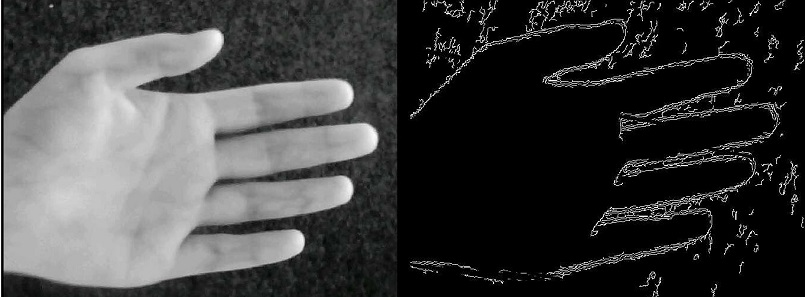
\includegraphics[scale=0.7]{figures/compare6.JPG}
\caption[Hough transform, detection of edges]{Hough transform, detection of edges}\label{fig:Compare6}
\end{figure}


\begin{figure}[H]
\centering
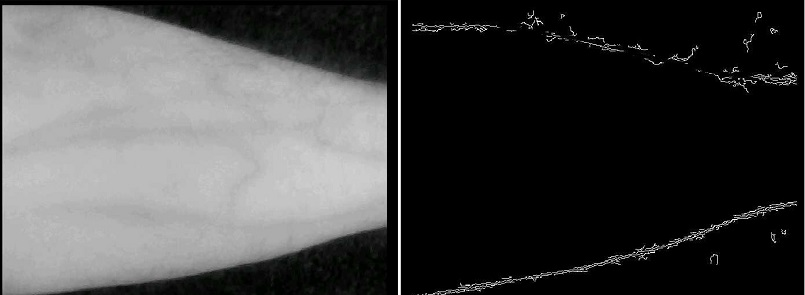
\includegraphics[scale=0.7]{figures/compare7.JPG}
\caption[Hough transform, failed detection of veins]{Hough transform, failed detection of veins}\label{fig:Compare7}
\end{figure}


\subsubsection{Image Processing: Laplacian Transformation}
The Laplacian of an image highlights regions of rapid intensity change and is therefore often used for edge detection. It can be considered as an equivalent measure of the second derivative in 2D.
Given $f$, a function of time, with value $f(t)$ at time $t$, the Laplace transform of $f$ is denoted $\widetilde {f} $ and it gives an average value of f taken over all positive values of $t$ such
that the value $\widetilde{f}(s)$ represents an average of $f$ taken over all possible time intervals of length $s$ \parencite{laplace}.

\begin{equation}
\mathcal{L}[f(t)]= \widetilde{f} (s) = \int_{0}^{\infty} e^{-st} f(t)dt,  s >0 
\end{equation}

The idea behind the Laplacian transformation is simple. If the change in a pixel in the second derivative is steep enough, it is marked as an edge pixel. Deciding that is done by calculating the zero crossings and that is when the slope changes direction from positive to negative or vice versa. That point is then the edge's location. 

Similar to the Hough transformation, the Laplacian transformation yielded insufficient results in detecting veins.



\begin{figure}[H]
\centering
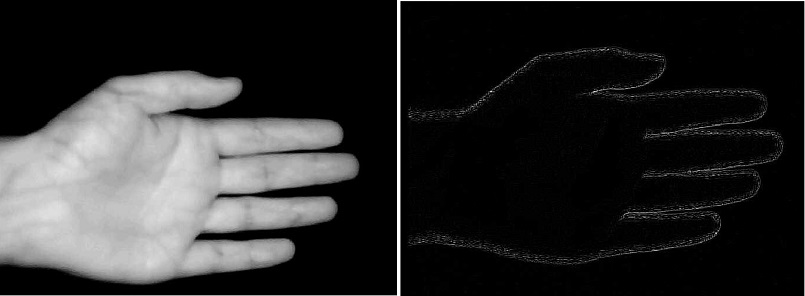
\includegraphics[scale=0.7]{figures/compare8.JPG}
\caption[Laplace transform, detection of edges]{Laplace transform, detection of edges}\label{fig:Compare8}
\end{figure}

\begin{figure}[H]
\centering
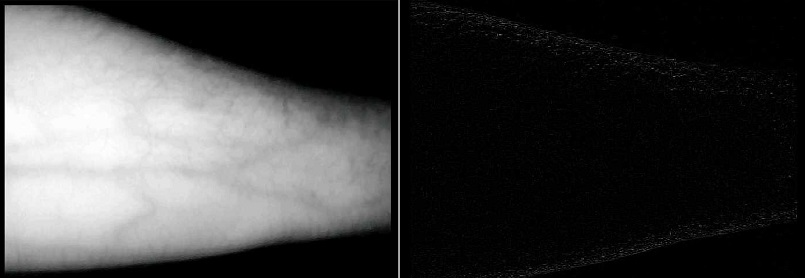
\includegraphics[scale=0.7]{figures/compare9.JPG}
\caption[Laplace transform, failed detection of veins]{Laplace transform, failed detection of veins}\label{fig:Compare9}
\end{figure}


\section{Application Work Modes}
From software point of view, the application can work under two modes: raw NIR images without image processing and adaptive thresholding.

\subsection{Raw NIR Images Mode}

The term “raw NIR images” refers to the fact that no image processing operation was performed on the images before showing them on the screen. As stated in previous chapters, images from the adjusted webcam are sent to the mobile device via a third-party library, the UVC Camera library. As the camera is adjusted, it can sense almost only NIR light and no visible light. These raw images are not purely raw from hardware point of view, as they are already manipulated through the NIR-pass filter. They appear to be transformed in the greyscale. For normal healthy patients with relatively light skin colour, showing raw NIR images can provide good visualization of the veins pattern. \autoref{fig:RawNirImage} shows an NIR image of the arm of a normal healthy male person. No tourniquet was used while taking these images.


\begin{figure}[H]
\centering
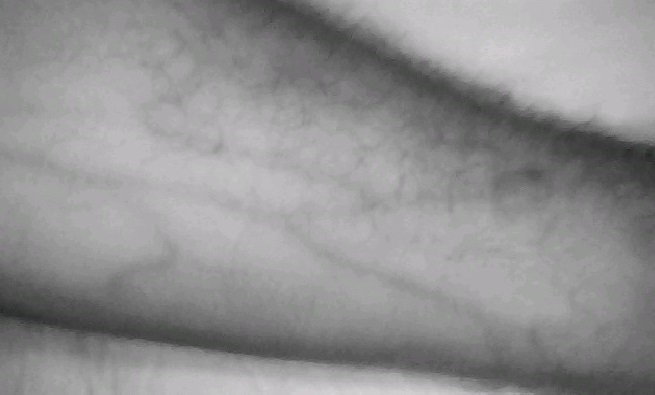
\includegraphics[scale=0.7]{figures/nir.JPG}
\caption[Raw NIR Image of an Arm with Good Vein Contrast]{Raw NIR image of the arm of a normal healthy male person.}\label{fig:RawNirImage}
\end{figure}

The \autoref{fig:RawNirImage} shows a good contrast of the vein on the arm. Localizing the vein depending on this image is then an easy task. However, raw NIR images don’t always show such good contrast without any processing. Many different factors could be responsible for poor contrast in raw NIR images such as body weight, skin colour and gender.  In the \autoref{fig:RawNirImage1}  shows an arm of a normal female person on the same setting, poor contrast is noticeable and the vein has barely darker colour than the surrounding area.
The result of venepuncture depending on images with such veins contrast will not be better than the traditional way of visual examination and palpation. The only remarkable difference between the two persons here is the gender. However, the gender factor is not necessarily the deciding factor. For another female person, vein contrast was as good as the contrast in \autoref{fig:RawNirImage}.

\begin{figure}[H]
\centering
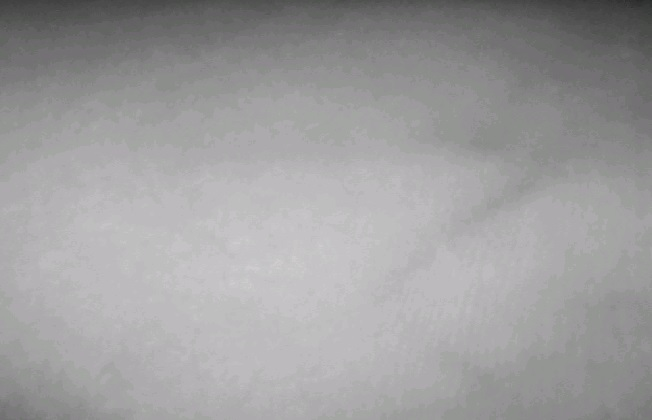
\includegraphics[scale=0.7]{figures/nirZein.JPG}
\caption[Raw NIR Image of an Arm with Poor Vein Contrast]{Raw NIR image of the arm of a normal healthy female person.}\label{fig:RawNirImage1}
\end{figure}

\subsection{Adaptive Thresholding Mode}
Because of poor vein contrast of raw NIR images in some cases, image processing can be of great benefit. Adaptive thresholding has given very good results in terms of performance and vein contrast.
\subsubsection{Image Segmentation}
Image segmentation is a fundamental process in many image, video, and computer vision applications. It is often used to partition an image into separate regions, which ideally correspond to different real-world objects \parencite{imageSeg}. It is the process of assigning a meaningful label to every set of pixels in the image so that these sets represent different segments. Like separating an object from the background or segmentation of multiple different objects in an image. Image segmentation is usually performed by identifying common properties between regions. Or, similarly, by identifying differences between them.

\subsubsection{Image Thresholding}

Image thresholding is the most common and simplest image processing approach to segment images. In general image thresholding aims to change pixel values depending on a threshold. For images in the greyscale, image thresholding yields binarized images, i.e. images that only has two colours. 

Let $f(x; y)$ be the grey value of the image at pixel in position $(x; y)$; then thresholding using threshold value $t$ transforms this image into a binary image $f'(x; y)$ as follows:

\begin{equation}
\mathcal{} f'(x; y)
  \begin{cases}
    0 & \text{if $f(x; y) \leq t$} \\

    255 & \text{otherwise}
  \end{cases}
\end{equation}

All pixels below the threshold $t$ are turned into 0 and all others that are above this threshold are turned into 255. The threshold as well as the two assigned pixel values can be adjusted based on application specification.

\subsubsection{Global Threshold}
Global thresholding approach can be used if the intensity distribution between the segments is very distinct. In this method, only a single value (global value) for the threshold for all pixels in the image is used. Threshold value should be then carefully selected and based on practical results. However, any changes in the lightning conditions or colours of the image could affect the thresholding drastically and misclassify big regions in the image. Because the dependence is on the colour intensity only, not on any relationships between the pixels. These effects get worse as the noise increases, because it’s more likely that a pixel’s intensity doesn’t represent the normal intensity in the region. 
Applying global thresholding on the NIR images has given very bad results. \autoref{fig:thresholdGlobal} shows a global thresholding result on the image in \autoref{fig:RawNirImage} using threshold value of 160.

\begin{figure}[H]
\centering
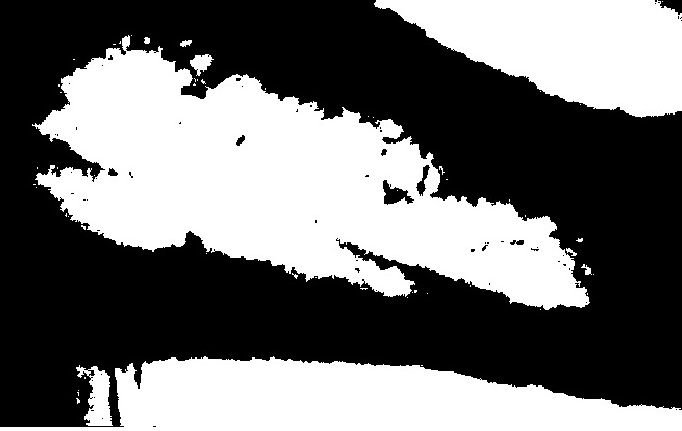
\includegraphics[scale=0.6]{figures/thresholdGlobal.JPG}
\caption[Global thresholding example]{Global thresholding on the image in \autoref{fig:RawNirImage}; threshold value: 160}\label{fig:thresholdGlobal}
\end{figure}

\subsubsection{Local (Adaptive) Threshold}
Another problem with global thresholding is that changes in illumination across the image may cause parts to be brighter and others darker. To overcome the global thresholding shortcomings, adaptive thresholding can be used. 
Unlike global image thresholding, local image thresholding uses multiple, local, thresholds for each region of the image. Finding the local threshold across the image regions depends on the fact that smaller image regions are more likely to have approximately uniform illumination, thus being more suitable for thresholding. Automatic calculation of local threshold for each pixel can be achieved in many approaches such as mean calculation and Gaussian methods. In both methods, the threshold is calculated for each pixel by taking the neighbouring pixels into consideration. Depending on their values, the threshold value of the pixel can then be decided.

\subsubsection{Local Threshold Calculation by Mean}
For each pixel at $(x; y)$, the threshold value $T(x; y)$ is the mean value of the neighbouring pixels of $(x; y)$ in an area of size $blockSize \times blockSize$ minus a correction constant $C$. 

Increasement of the block size results in more neighbouring pixels taken into consideration while calculating the threshold value for each pixel. Determining the block size is deciding factor for the quality of the results. Luckily, the block size can be set based on visual assessments of the results and doesn’t need to be reconsidered for other images in the same setting. 

\begin{figure}[H]
\centering
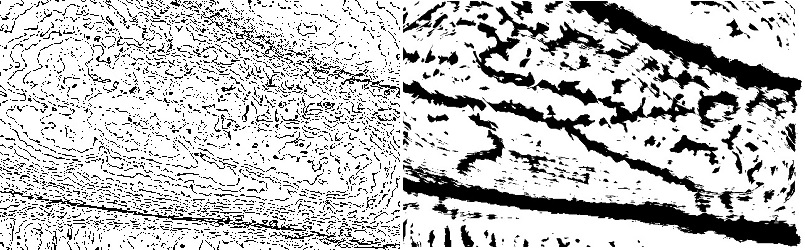
\includegraphics[scale=0.8]{figures/compare1.JPG}
\captionsetup{justification=centering}
\caption[Effect of block size on mean adaptive thresholding]{Effect of block size on mean adaptive thresholding;\\C of both: 2; block size: left 7, right 41}\label{fig:compare1}
\end{figure}

The correction constant is a constant value that is subtracted from each threshold. Increasing this constant reduces noise but, of course, might result into loss of some desired details. Normally, this constant is positive, but it can be assigned a negative value as well.

\begin{figure}[H]
\centering
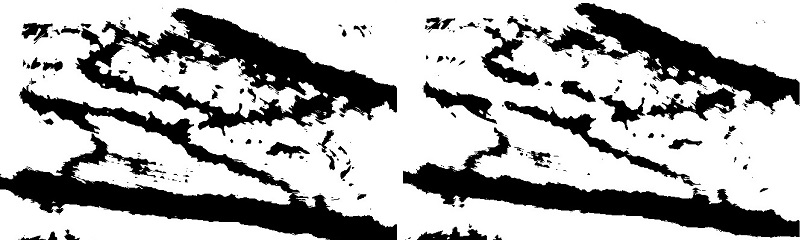
\includegraphics[scale=0.8]{figures/compare2.JPG}


\caption[Effect of correction constant on mean adaptive thresholding]{Effect of correction constant on mean adaptive thresholding; block size for both: 91; C: left 0, right 2; Partial loss of details is noticeable}\label{fig:compare2}
\end{figure}

\subsubsection{Local Threshold Calculation by Gaussian}
For each pixel at $(x; y)$, the threshold value $T(x; y)$ is the is a weighted sum (cross-correlation with a Gaussian window) of the neighbouring pixels of $(x; y)$ in an area of size $blockSize \times blockSize$ minus a correction constant $C$. 

The main approach is similar to the previous approach in mean calculation. The only difference is the relation between the pixels or pixel regions. In mean calculation approach, all pixels in a surrounding area of size $blockSize \times blockSize$ have the same weight in the calculation, and thus, they have the same effect on the final threshold value. In Gaussian calculation approach, cross correlation of the area surrounding each pixel is used to assess how similar this area with each neighbouring area. A weighted sum is then calculated.

Cross-Correlation $g(i ;j)$ of two functions $f(x ;y)$ and $ h(x; y)$ can be calculated as follows:

\begin{equation}
g(i;j) = f(x; y) \otimes h(x; y) = \iint_{-\infty}^{+\infty} f(x; y) h(i - x; i - y) dx dy
\end{equation}
 
Similar to mean adaptive thresholding, block size and correction constant have impact on the result’s quality.  

\begin{figure}[H]
\centering
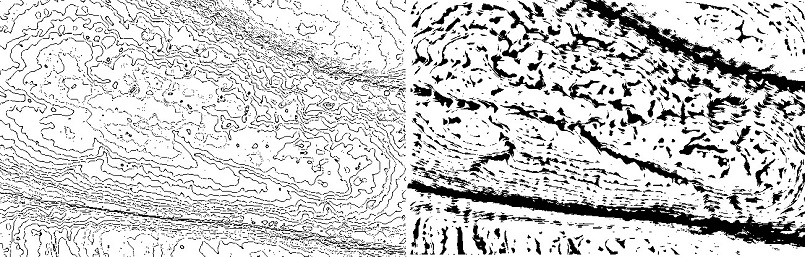
\includegraphics[scale=0.8]{figures/compare3.JPG}
\captionsetup{justification=centering}
\caption[Effect of block size on Gaussian adaptive thresholding]{Effect of block size on Gaussian adaptive thresholding;\\C for both: 2; block size: left 7, right 41}\label{fig:compare3}
\end{figure}


\begin{figure}[H]
\centering
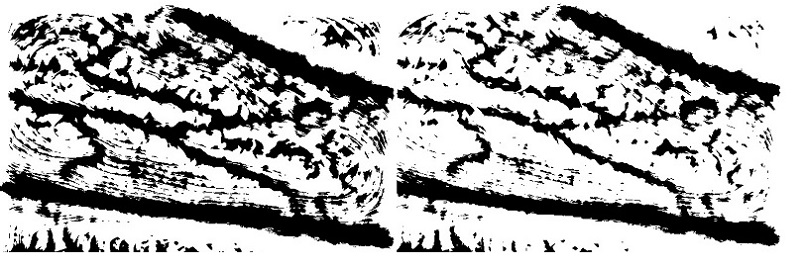
\includegraphics[scale=0.8]{figures/compare4.JPG}
\captionsetup{justification=centering}

\caption[Effect of correction constant on Gaussian adaptive thresholding]{Effect of correction constant on Gaussian adaptive thresholding;\\ block size for both: 91; C: left 0, right 2}\label{fig:compare4}
\end{figure}

\subsubsection{Median Filter}
In addition to the correction constant, image noise removal can be achieved by applying a filer after getting the adapt thresholding result. A good candidate here is the median filter. Similar to the adapt thresholding, median filter is a nonlinear image processing operation. The median filter is an effective method that can, distinguish out-of-range isolated noise from legitimate image features such as edges and lines. Noise reduction is done replacing each pixel with the median of all pixels in a defined size neighbourhood $w$ of the given pixel. 

\begin{equation}
f(x; y) = median \{g(x; y) | (x; y)\in w   \}
\end{equation}


\begin{figure}[H]
\centering
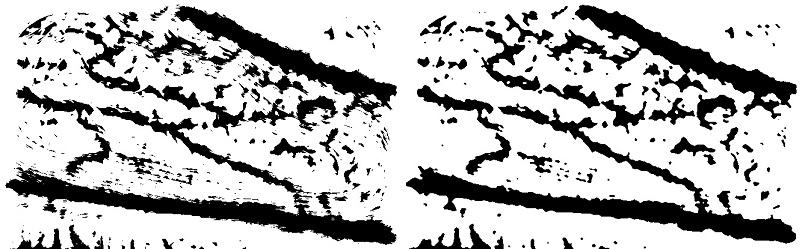
\includegraphics[scale=0.8]{figures/compare5.JPG}
 

\caption[Median filter]{Median filter; left: result of Gaussian adaptive thresholding with block size: 91, C: 2; right: result of applying median filter with kernel size: 4; Noise is reduced with no details loss}\label{fig:compare5}
\end{figure}


Moreover, the median filter is better than the average filter, which calculates the average of pixels in the neighbourhood and replaces every pixel with it. Because in average filter, a single pixel with a very unrepresentative value can significantly affect the average value of all the pixels in its neighbourhood. 


\section{Application Structure}
The software application is basically an android application composed of two layers: the native layer, written in C++ and the Java layer. 
The Java layer includes user interface (UI) components of the application and all application business logic. 
The C++ layer is responsible for communicating with the camera as well as for image processing of raw images coming from the camera using open computer vision library (OpenCV).

Because compiled Java code runs on the Java virtual machine (JVM) which is a part of the Java runtime environment (JRE). Whereas compiled C++ runs directly on the operating system (OS), a bridging component Between the two layers is needed.
The Java native interface (JNI) allows the two layers to interact with each other. It is a Java feature that allows Java code to call native applications and libraries written in languages such as C, C++ and Objective-C.

The \autoref{fig:applicationArchitecture} below shows the application high-level architecture.


\begin{figure}[H]
\centering
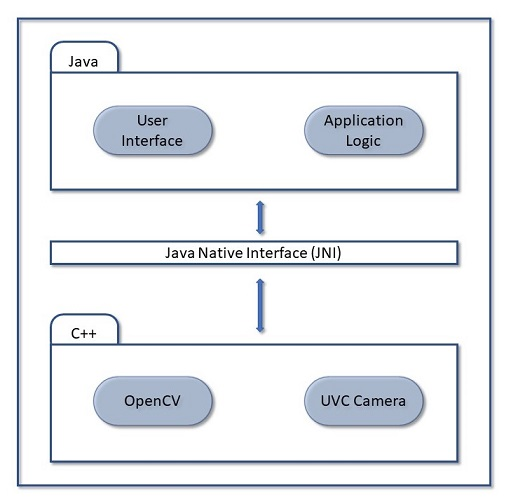
\includegraphics{figures/applicationArchitecture.JPG}

\caption[Application architecture]{Application architecture}\label{fig:applicationArchitecture}
\end{figure}
\subsection{C++ Layer}

Using native C++ has many benefits in terms of high performance and compatibility.
C++ is a highly flexible and adaptable language. Since its creation, it has been used for a wide variety of programs including firmware for micro-controllers, operating systems, applications, and graphics programming \parencite{cpp}.

Android offers a good and easy-to-use C++ Integration via the JNI. In fact, Android Studio (current version 3.2.1) offers an option to include C/C++ support when creating a new application. Native C++ classes as well as corresponding JNI methods and Java classes are automatically created. Even for an existing project, importing a native C++ library or adding C++ code can be done easily on Android Studio.

One big advantage of using C++ is the cross-platform feature which the language offers. Code can be written on any environment and seamlessly run on other environment. During development, it was very inconvenient to run and test directly on a mobile device. Because of time loss in building the android application, packaging it and installing the APK file on the device. Instead, development, algorithms calibration and tests were performed directly on Linux using a desktop and the CLion IDE.

Written in C++, this application layer encompasses the UVC Camera library which allows the application to communicate with the camera as well as the native image processing module, the OpenCV module.



\subsubsection{USB Video Class}

USB Video Class (UVC) describes the capabilities and characteristics of video streaming devices. It is widely used, such as desktop video cameras or webcams, digital camcorders, still-image cameras, and so forth. USB Video Class (UVC) is a standard class specification that standardizes video streaming functionality on the USB. It enables devices like webcams, digital camcorders, analogue video converters, analogue and digital television tuners etc to connect seamlessly with host machines. UVC supports streaming multiple video formats and provides structures for describing the functionalities of the video device to the host and defines USB requests to control different parameters of the device and characteristics of the video stream. It also provides flexibility for a video device to support multiple video resolutions, formats and frame rates, which highly influences the bandwidth negotiation between the device and the host \parencite{uvc}.

\subsubsection{UVC Camera Library for Android}
Many OS platforms have native support for UVC drivers which greatly reduces the time required for developers to connect UVC devices. Unfortunately, android doesn’t offer such a support, therefore, to connect a UVC device such as a webcam, the device driver must be written by the developer. 
Nevertheless, third-party and open source libraries offer good alternative solution for the UVC device drivers. An open source library to access to UVC webcams on non-rooted Android device called UVCCamera was used in this project \parencite{uvcCamera}. The library works on minimum android version 3.1 or later (API >= 12), but Android 4.0(API >= 14) or later is recommended. Of course, to use it, many configurations and tuning steps were needed. Especially, due to the fact that no enough documentation is available.


\subsubsection{Open Computer Vision Library}
OpenCV is written in C and C++ and runs under Linux, Windows and Mac OS X. OpenCV was designed for computational efficiency and with a strong focus on realtime applications and can take advantage of multicore processors. One of OpenCV’s goals is to provide a simple-to-use computer vision infrastructure that helps people build fairly sophisticated vision applications quickly \parencite{openCv}.

OpenCV offers support for common image processing algorithms. Adaptive thresholding, for example, is implemented in this project using OpenCV. The video captured by the camera is a sequence of images. Each image can be represented as a matrix of numbers. Image processing algorithms tend to be quite computationally heavy, therefore, OpenCV has its own type to represent arrays, namely the $Mat$ class. $Mat$ can be used to store real or complex-valued vectors and matrices, grayscale or colour images and more. It is optimized to be passed to the functions without making unnecessary copies. Each $Mat$ object has a header, the matrix that holds the data may be shared between two instances of them by having their matrix pointers point to the same address. Moreover, the copy operators will only copy the headers and the pointer to the large matrix, not the data itself \parencite{openCv1}.


\subsubsection{Android NDK}


The Android NDK is a companion toolset for the Android Software Development Kit (SDK), designed to augment the Android SDK to allow implementation of performance-critical portions of android applications using machine code-generating programming languages like C, C++, and assembly \parencite{ndk} or to access physical device components, such as sensors and touch input. 
The NDK builds the native shared libraries, or $.so$ files, from C/C++ source code as well as the native static libraries, or $.a$ files, which can be linked into other libraries.


\subsection{Java Layer}

The Java layer includes the user interface (UI) components and all application business logic.
The compiled Java code along with any data and resource files required by the application is bundled by the android asset packaging tool (AAPT) tool into an android package, an archive file marked by an .apk suffix.

While the core functions in the UVC Camera library are written in C/C++, the library offers a Java interface and it has many modules written in Java. Therefore, here, the Java layer, additionally to the application itself, addresses some of the library parts that are written in Java and used in the application.



\subsubsection{Permissions: USB Host}
By default, Android does not allow an application to access the devices connected to the USB  port. To enable an application to interact with a the UVC camera directly connected by OTG cable, this functionality must be declared by adding the \texttt{<uses-feature android:name="android.hardware.usb.host"/>} tag in the manifest section in \texttt{ AndroidManifest.xml}. 

\subsubsection{USBMonitor}

This class manages the USB connection via the OTG port on the android device. It notifies the application when a USB device is attached, detached, connected or disconnected. Principally, the USB, and, therefore, the OTG, protocol allows connection of multiple peripherals. Of course, a USB hub is then needed. The USBMonitor class provides the application with a list of connected devices as well as each device’s vendor ID, product ID, device class and subclass, device protocol and more hardware-related information.

\subsubsection{Permissions: Open GL}

OpenGL ES (Open Graphics Library for Embedded Systems) is an API to graphics hardware. The API consists of a set of several hundred procedures and functions that allow a programmer to specify the shader programs, objects and operations involved in producing high-quality graphical images, specifically color images of three-dimensional objects \parencite{openGl}.
Android includes support for high performance 2D and 3D graphics with the OpenGL ES. Similar to USB host permission, adding  \texttt{<uses-feature android:glEsVersion="0x00030000"/>} tag to include OpenGL ES support is needed. This tells android to expect the version 3 of OpenGL ES.

\subsubsection{ImageProcessor}

The image processor class is part of the OpenCV Java-wrapper. It offers frame-based image processing capabilities using OpenCV. After configured and set up, whenever a frame arrives from the camera to the UVC Camera module, the corresponding activity calls the $doProcess$ method in the image processor class. The image processor Java class calls another C++ image processor class via the JNI. The later receives an image then by reference, processes it and sends it back to the Java side. After that, the Java image processor callback $onResult$ is called to return the processed frame to the activity. The fast succession of frames (about 30 fps) makes up the processed video.


\subsubsection{Android SurfaceView}
After the frame has been processed in the image processor class, it is then sent back to the application to show it on the screen. Drawing on Android activities is performed by the same UI thread which is also used for all user interaction. Therefore, using this thread to draw the processed, or even raw, frames is not feasible and will cause the application to freeze. Instead, android offers another view type, the SurfaceView, which can be drawn on a background thread without affecting the user experience. Therefore, results are drawn on a SurfaceView. 
However, SurfaceViews have some limitations. The main limitation is that they are not hardware accelerated, while most of operations on normal Views are hardware accelerated using OpenGL ES. Another limitation is that, SurfaceViews have dedicate surface buffer while all Views share one surface buffer. In another words, SurfaceViews cost more resources. Despite its limitations, practically, SurfaceView is sufficient for this project goals due to the small frame size and low resolution. 



\subsubsection{Control of Algorithm Type and its Parameters}

The application offers simple UI components to control the image processing algorithm type or its parameters. For example, as explained earlier, adaptive thresholding can be applied with or without the median filter. Selection of this option is done in the Java side through UI components and then sent to the C++ side via the JNI. Similarly, algorithm parameters can be changed the same way. A slider to adjust the kernel size of the median filter is shown on the screen. The kernel size is stored as a local variable in the C++ image processor class. During every image processing operation, i.e. on every frame, this variable is read and then used by the algorithm. When the user changes the slider’s value, the android activity calls a method in the Java image processor to change the kernel size, which in turn calls a corresponding method in the C++ image processor. Finally, the value is changed in that class and stored there. Java stores no information about the algorithm type or parameters and they are queried from the C++ side whenever they are needed. 






 
